\documentclass[11pt]{article}

% Change "review" to "final" to generate the final (sometimes called camera-ready) version.
% Change to "preprint" to generate a non-anonymous version with page numbers.
\usepackage[preprint]{acl}

\usepackage{pgfplots}

\usepackage{multirow}
\usepackage[table]{xcolor}

% Standard package includes
\usepackage{times}
\usepackage{latexsym}
\usepackage{hyperref}

% For proper rendering and hyphenation of words containing Latin characters (including in bib files)
\usepackage[T1]{fontenc}
% For Vietnamese characters
% \usepackage[T5]{fontenc}
% See https://www.latex-project.org/help/documentation/encguide.pdf for other character sets

% This assumes your files are encoded as UTF8
\usepackage[utf8]{inputenc}

% This is not strictly necessary, and may be commented out,
% but it will improve the layout of the manuscript,
% and will typically save some space.
\usepackage{microtype}

% This is also not strictly necessary, and may be commented out.
% However, it will improve the aesthetics of text in
% the typewriter font.
\usepackage{inconsolata}

%Including images in your LaTeX document requires adding
%additional package(s)
\usepackage{graphicx}

\usepackage[normalem]{ulem}
\usepackage{cleveref}


% when resolved, either comment in text, or change this repo to:
% \def\XXX#1{} % which hides all XXX 
\def\XXX#1{\textcolor{red}{XXX #1}}

% similarly with this
\def\repl#1#2{\textcolor{orange}{\sout{#1}}\textcolor{blue}{#2}}



% If the title and author information does not fit in the area allocated, uncomment the following
%
%\setlength\titlebox{<dim>}
%
% and set <dim> to something 5cm or larger.

% previous title:
%\title{Repurposing a Small Offline End-to-End Model for Simultaneous Speech Translation in IWSLT 2026}
\title{A Pocket Offline Model for Simultaneous Speech Translation as CUNI Submission to IWSLT 2026}

%Author information can be set in various styles:
%For several authors from the same institution:
%\author{Aziz Sharipov Ortega \and Dominik Macháček \\
%        Address line \\ ... \\ Address line}

% For authors from different institutions:
% \author{Author 1 \\ Address line \\  ... \\ Address line
%         \And  ... \And
%         Author n \\ Address line \\ ... \\ Address line}
% To start a separate ``row'' of authors use \AND, as in
% \author{Author 1 \\ Address line \\  ... \\ Address line
%         \AND
%         Author 2 \\ Address line \\ ... \\ Address line \And
%         Author 3 \\ Address line \\ ... \\ Address line}

\author{Aziz Sharipov Ortega \\
  Charles University, MFF \\
  \texttt{azdisharipov@gmail.com} \\\And
  Dominik Macháček \\
  Charles University, MFF, ÚFAL \\
  \& University of Edinburgh \\
  \texttt{machacek@ufal.mff.cuni.cz} \\}

% \author{
%  \textbf{Aziz Sharipov Ortega\textsuperscript{1}} \And
%  \textbf{Dominik Macháček\textsuperscript{1,2}}
% \\
% \\
%  \textsuperscript{1}Charles University,
%  \textsuperscript{2}University of Edinburgh,
% \\
%  \small{
%    \textbf{Correspondence:} \href{mailto:email@domain}{email@domain}
%  }
% }

\begin{document}
\maketitle
\begin{abstract}
% This paper describes two Charles University’s submissions to the Simultaneous Speech Translation Task of the IWSLT 2026. \XXX{TODO}
% We have two main goals.

% We repurpose an offline direct speech-to-text translation model Canary-v2-1B for simultaneous translation, and submit it to IWSLT 2026 Simultaneous Speech Translation Shared task for Czech to English and English to German and Italian. 

We implement a direct speech translation model Canary for simultaneous translation with 
AlignAtt simultaneous policy. We focus on Nemo toolkit with the recent state-of-the-art foundation model Canary-1B-v2 that has only one billion of parameters, which is suitable for small pocket devices. 
This is a CUNI submission to IWSLT 2026 Simultaneous Speech Translation Shared task on Czech to English and English to German and Italian.

The strengths of our system are: (1) high translation quality, overperforming similarly sized baselines both in low- and high-latency regimes in both computationally unaware and aware simulations; (2) low computational requirements, as the neural model that we use has only 1B parameters; (3) multilinguality -- support of 25 source and 25 target languages.
\end{abstract}

\section{Introduction}
In this paper, we describe a submission of the Charles University (CUNI) to IWSLT 2026
Simultaneous Speech Translation Task \cite{anastasopoulos-etal-2026-findings}. Our system is built on top of Canary-1B-v2\footnote{Throughout this paper, we usea simple term \textit{Canary} to refer to the \textit{Canary-1B-v2} model}, even though technically \textit{Canary} is a family of models.}\citep{sekoyan2025canarybv} with AlignAtt \citep{papi2023alignatt} simultaneous policy. Following  SimulStreaming \cite{machacek-polak-2025-simultaneous}, the highest performing submission in IWSLT 2025 \cite{agostinelli-etal-2025-findings}, we also use Silero Voice Activity
Detection (VAD) in the pipeline to reduce noise and hallucination in non-speech periods of audio. We validate the latency of our systems in computationally unaware simulation, and submit also a version for computational aware simulation.

One of the strenghts of our system is high multilinguality. The Canary model supports 25 source and 25 target languages for direct translation, which overlaps with three language pairs of IWSLT 2026 we focus on: Czech to English, English to German, and English to Italian. The model is also very small and high quality. It has only 1B parameters, making it operational even on small mobile devices.\footnote{\url{https://www.siliconflow.com/articles/en/best-lightweight-LLMs-for-mobile-devices} suggests that even 8B-parameter models are suitable for mobile devices.}
%, such as contemporary high-end smartphones, such as models from the Gemma family \citep{manik2026gemma}.

%Repurposing offline models for use in simultaneous mode is not a novelty and has been successfully applied in practice before \citep{machacek-polak-2025-simultaneous,papi-etal-2022-simultaneous}. However, with the release of Canary-1B-v2, an ultra-light automatic speech translation (AST) and speech recognition (ASR) model, this approach has become more attractive as it potentially allows real-time translation and speech recognition system to be deployable on pocket devices.

We follow the approach of repurposing offline speech translation models for simultaneous mode because it has been shown as a simple, effective, and well-performing strategy, e.g.\ in \citet{papi-etal-2022-simultaneous} and in \citet{machacek-polak-2025-simultaneous}. The benefits of high quality, multilinguality, flexibility, and robustness often overweight the limitations such as hallucination on partial source sentences, not using left-only context, or repeated encoding of the whole source buffer with every new incoming chunk, that can be avoided by specific simultaneous methods, which usually require costly training, e.g. for stability on source prefixes \cite{niehues18_interspeech}, for learning to wait or translate \cite{Koshkin2026StreamingTA}, or  specific simultaneous models \cite{arivazhagan-etal-2019-monotonic,kyutai2025hibiki}.
We observe a higher demand for offline speech translation than for simultaneous. New, higher quality and diverse offline models are becoming available, but there is a gap in flexible and robust implementations that enable processing any offline model in simultaneous mode. This is a gap that we aim to fill with this work. 

Our primary goal is therefore to pioneer Canary usage in simultaneous mode and evaluate it against state-of-the-art systems, to test whether Canary in simultaneous mode can be used in practical applications and as a baseline in future research.

 %last year winner submission.


We conclude we have reached the main goal. The results show competitive and in some cases even superior performance to state-of-the-art baselines while being much smaller in size. Our results show improvements by over 4-5 BLEU points over the organizers' baseline on English to German and Italian and 5-8 BLEU points for Czech to English over the IWSLT 2025 best performing system \citep{machacek-polak-2025-simultaneous}.

The paper is structured as follows: in the \Cref{sec:background}, we introduce the core model and policies and provide a relevant background. In \Cref{sec:implementation}, we dive into implementation details of our submission, while \Cref{sec:dev} serves as a detailed description of the frameworks and evaluation metrics used, which we then follow by the evaluation result in \Cref{sec:results}. Finally, we wrap up the paper with a conclusion and limitations regarding the implementation.


\section{Background}
\label{sec:background}
\paragraph{Canary-1B-v2} \citep{sekoyan2025canarybv} is a strong multitask speech transcription and translation model with state-of-the-art performance. It outperforms \textit{whisper-large-v3} \citep{radford2022whisper} and \textit{seamless-m4t-medium} in automatic speech recognition (ASR) and automatic speech translation (AST) tasks, and on some datasets is even superior to s\textit{eamless-m4t-v2-large}, which is twice as large in size. Additionally, it supports injecting context in the decoder prompt to bias the prediction with in-domain context, and timestamping. Unlike Whisper, Canary does not need to work with fixed size audio inputs and was instead trained to support audios in 0 to 40 seconds range, which makes it a perfect candidate for simultaneous adaptation.

\paragraph{AlignAtt} \citep{papi2023alignatt} is a simultaneous
policy. This policy idea is to use the cross-attention layer in the decoder to omit the suffix of hypothesis after the first token that attends to a predefined frame threshold. It has been shown to work well in long-form translation \cite{papi-et-al-2024-streamatt} and with Whisper \citep{wang2024simulwhisper,machacek-polak-2025-simultaneous}, but has not been previously applied on Canary.

\paragraph{Sliding window} \citep{sen2022simultaneous} is another simultaneous policy. Its core idea is to re-translate a window of audio input, use longest common subsequence with the previous translation to avoid repeating, and sliding the window with newly available audio chunk. Although being outperformed by AlignAtt, the only available implementation of Canary in simultaneous mode by \citet{gaido2025simulstream} uses this approach. We use it as a baseline for comparison to our system.

%\paragraph{Offline models in simultaneous mode}


%An approach of applying simultaneous decoding policy on offline model creates very highly performing simultaneous systems, although they are not trained or designed for incomplete source and target, left-only context, or detecting when to wait for context or translate. And even when the offline encoder in simultaneous mode very inefficient, encoding the whole 30-second audio buffer repeatedly with every newly incoming chunk, the offline computational frameworks, including Nemo, are already very fast, so they can be usable in simultaneous mode even without specific methods that reduce this inefficiency.



%\XXX{why Canary (and Nemo): better than Whisper/Seamless, small = efficient, direct speech-to-text translation, multilingual}

% \XXX{why AlignAtt for Nemo} Motivation: new SoTA offline models are there, overperforming previous SoTA models WHisper and Seamless (any ref. for that)
% but simple naive simultaneous implementations using re-translation, naive chunking, or LocalAgreement are bad. (re-translation flickers, naive VAD chunking is slow or low-performing, LocaAgreement is slow).
% AlignAtt policy is there, but it's hard to implement as Nemo was not providing access to attention before we started to work on it.






\section{Implementation}
\label{sec:implementation}
Let us describe the details of the implementation of our systems and the end-to-end long-form speech-to-text processing pipeline. %What follows applies to all AST directions in the scope of the submission. % 

\paragraph{Simulation frameworks}
There are two frameworks for end-to-end simulation of speech-to-text simultaneous systems on pre-recorded audio that also allow integration of new models: the earlier introduced is SimulStreaming \cite{machacek-polak-2025-simultaneous} and the latter Simulstream \citep{gaido2025simulstream}. We use primarily SimulStreaming because it provided a robust implementation of SileroVAD \cite{Silero_VAD}, % \url{https://github.com/snakers4/silero-vad}, 
a streaming voice activity detection that filters non-voice parts of the input audio and allows to save computational power on processing empty input, while also avoiding potential hallucinations.

Since IWSLT 2026 task required Simulstream for computational aware evaluation, we finally transfer our Canary implementation to Simulstream to enable it. However, in case of differences, we consider our SimulStreaming implementation as the primary. %Both frameworks provide comparable input format for the evaluation tool OmniSTEval. Therefore, we could use the organizers' baseline Simulstream baseline systems for    

% \paragraph{SimulStreaming}
% The primary framework for simultaneous translation during development was chosen to be SimulStreaming available at \url{https://github.com/ufal/SimulStreaming}, since it already incorporated VAD system, which filters non-voice parts of the input audio and allows to safe computational power on processing empty input, while also avoiding potential hallucinations.

% \paragraph{Simulstream} We make use of pre-implemented canary simultaneous architecture using sliding-window policy, provided by the organizers' simulstream\citep{gaido2025simulstream} framework, to compare our results against. We finally transfer our implementation of Canary to simulstream as our computationally aware submission. 

\paragraph{Adapting Nemo} It was not straightforward to directly apply the AlignAtt policy to Canary model in Nemo, since the API did not support decoder forced prefix\footnote{The approach is described clearly in this thread \url{https://github.com/openai/whisper/discussions/117\#discussioncomment-3727051}} injection required for the incremental output. Hence, we highlight our contribution to the Nemo's speech framework \citep{Harper_NeMo_a_toolkit} that allows for this core incremental concept to be used with Canary. With our contribution, now the prefix can be provided as an optional initial prompt to the decoder. Additionally, we fixed the bug in the cross-attention outputs for the beam decoder strategy, which allowed us to get deterministic dimension outputs and map the cross-attention scores to their respective output tokens.

\paragraph{Processing loop} Our audio processing pipeline follows the stages of prototypical systems described in \citet{papi-etal-2025-real}, Section 3. We keep the same numbering of steps:

\begin{enumerate}
\item[1.-2.] Audio acquisition and segmentation using VAD is identical to SimulStreaming. Refer to \citet{machacek-polak-2025-simultaneous}, Section 3.

\item[3.] Speech buffer update. The incoming chunk, which has \textit{MinChunkSize}\footnote{We mark system parameters with italics.} seconds if the end of voice is not detected, or less otherwise, is concatenated with the speech buffer.

\item[4.] Hypothesis generation. Canary is an attention based encoder-decoder (AED) model. When audio is inputted, it is first encoded by the encoder. Then an initial prompt is passed to the decoder, which contains information about the source and target languages, decoder forced-prefix if any is in the buffer, as well as some other special tokens that affect final output, but are not relevant in the context of implementation, for example, whether to use timestamps. Then the model decodes the target as long as the AlignAtt policy allows. If any part of a word is inside the AlignAtt's frame threshold, the word is removed from the output. If the current chunk is not final, the decoding continues until the most attended source frame is close to the end of the audio, which is indicated by the \textit{Frames} parameter. In case the current chunk is final, we do not apply AlignAtt and output the whole generated sequence. 

\item[5.] Audio and context buffers. We use the following two buffers: (1) source audio buffer, which accumulates latest 30 seconds of audio in raw form. We note that although storing the mel-features instead of raw form is more efficient, as it skips the additional preprocessing step on every new chunk, we implement a simpler buffer as we were more focused on the computationally unaware scenario, and (2) forced decoding target buffer that contains the stable part of the hypothesis that was decoded from current audio buffer.

If the audio buffer has length of 30 seconds or more, we remove the first speech chunk from the source audio buffer. At the same time, we discard the text that was decoded with the first chunk from forced decoding. After shifting the buffer, it may happen that the audio is not entirely parallel to the forced decoded target buffer, but the results show that the model performs well with that. We leave possible improvement for further work.


\end{enumerate}

\section{Development}
\label{sec:dev}
\paragraph{Dev sets} For English-German and English-Italian directions, we use the MCIF \citep{papi2025mcif} dataset, as provided by the IWSLT 2026 organizers. For Czech-to-English direction, we use the
IWSLT 2026 dev set, which cosists of meetings of the Czech Chamber of Deputies.

\paragraph{MT metrics}
In our initial development, we relied on BLEU \cite{papineni-etal-2002-bleu} and ChrF \citep{popovic-2015-chrf} as our guiding quality scores with more emphasis on ChrF. However, for selecting the final system candidates, we used COMET-XL \citep{guerreiro-etal-2024-xcomet} as it is the main MT quality metrics for IWSLT 2026.
\paragraph{Latency metrics}
We use computationally unaware LongYAAL \citep{polk2025better} to select best hyper-parameters in the low- and high-latency ranges (2 and 4 seconds respectively).



\section{Results}
We evaluate our systems on the MCIF dev set for English-to-German and English-to-Italian, and on the IWSLT 2026 dev set for Czech-to-English. We compare against the following baselines: (1) the organizers' cascade baseline, which consists of a local agreement ASR component followed by a neural MT model(\textit{Qwen3-ASR-1.7B}\citep{shi2026qwenasr} and \textit{Qwen3-4B-Instruct-2507}\citep{yang2025qwen} respectively), (2) the Canary sliding window system as implemented in Simulstream, (3) Canary in offline mode, and finally (4) Simul-Streaming for Czech to English direction.

\paragraph{Metric scores and comparison}

\Cref{tab:dev_compare} reports our main results for the English-to-German and English-to-Italian directions. Our Canary with AlignAtt system outperforms the organizers' baseline across all four configurations -- high and low latency for both language pairs -- on BLEU, chrF, and XCOMET-XL. The improvements are most pronounced in the high-latency regime, where we gain over 4 BLEU points on English-to-German and more than 6 BLEU points on English-to-Italian. Notably, this holds even when comparing against the strongest organizers' baseline configuration that uses transcript context -- our system outperforms it on all quality metrics in the high-latency regime for both language pairs. In the low-latency regime, the quality gains are more modest on BLEU and chrF, especially for English to German direction, where the system falls behind the baseline, but XCOMET-XL consistently favors our system.

\begin{figure}[t]
    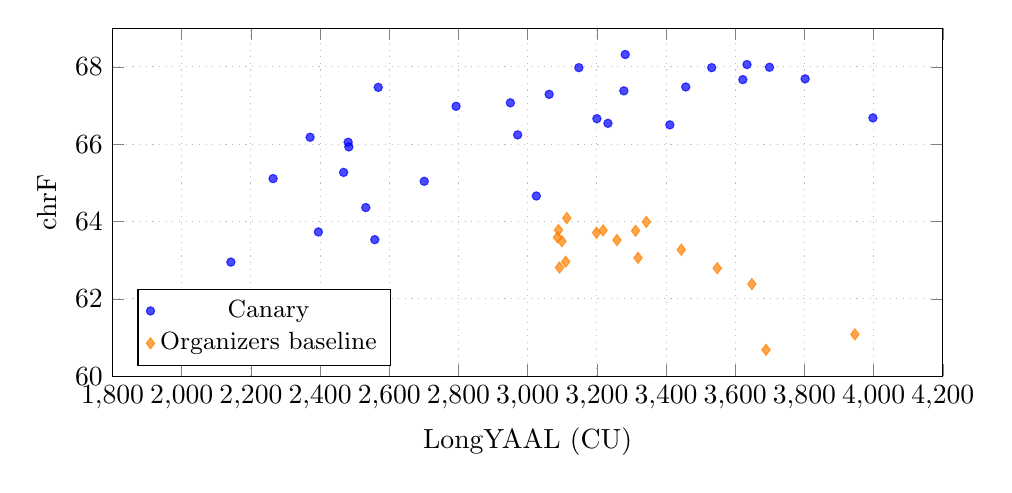
\begin{tikzpicture}
        \begin{axis}[
            width=\columnwidth,
            height=6cm,
            xlabel={LongYAAL (CU)},
            ylabel={chrF},
            xmin=1800, xmax=4200,
            ymin=60, ymax=69,
            legend pos=south west,
            legend style={font=\small, legend columns=1},
            grid=major,
            grid style={dotted},
        ]
        \addplot[only marks, mark=*, mark size=1.5pt, color=blue, opacity=0.7] coordinates {
            (2368,60.68) (2024,60.99) (2162,61.47) (2017,61.72)
            (2142,62.95) (2558,63.53) (2395,63.73)
            (2532,64.36) (3025,64.66) (2701,65.04) (2264,65.11) (2468,65.27)
            (2483,65.93) (2481,66.05) (2371,66.18) (2971,66.24) (3411,66.50)
            (3232,66.54) (3200,66.66) (3998,66.68) (2793,66.98) (2950,67.07)
            (3062,67.29) (3278,67.38) (2568,67.47) (3457,67.48) (3622,67.67)
            (3802,67.69) (3148,67.98) (3532,67.98) (3699,67.99) (3634,68.06)
            (3282,68.32)
        };
        \addlegendentry{Canary}

        \addplot[only marks, mark=diamond*, mark size=2pt, color=orange, opacity=0.7] coordinates {
            (3351,57.83) (3661,59.59) (3689,60.68) (3946,61.08) (3648,62.38)
            (3548,62.79) (3092,62.81) (3110,62.96) (3319,63.06) (3444,63.27)
            (3099,63.49) (3258,63.52) (3086,63.59) (3199,63.71) (3312,63.76)
            (3218,63.77) (3089,63.78) (3343,63.99) (3113,64.09)
        };
        \addlegendentry{Organizers baseline}

        \end{axis}
    \end{tikzpicture}
    \caption{English-to-Italian dev chrF vs.\ LongYAAL (CU) for Canary vs.\ the organizers baseline. Each blue point represents one Canary candidate from the search of \textit{MinChunkSize} and \textit{Frame} parameters. Orange points represent the organizers baseline system with grid-search for \textit{segment-length} and \textit{step-length}} 
    \label{fig:canary-baseline-enit}
\end{figure}

\Cref{fig:canary-baseline-enit} further illustrates the quality-latency trade-off on English-to-Italian. Notice that since our system has two parameters that influence latency-quality without any clear relation, it is not possible to plot the system candidate as a line, as it is typically done with other policies. Our Canary system dominates the organizers' cascade baseline across the entire latency range, achieving higher chrF at comparable or lower latency.

\label{sec:results}

\Cref{tab:dev_compare} additionally reports the scores of the Simulstream authors' Canary sliding window implementation, using the configuration they provide as default (chunk 2s, window length 12, matching threshold 0.1). Our AlignAtt-based system substantially outperforms this re-translation approach: on English-to-German, we gain over 8 BLEU points in the high-latency regime, and on English-to-Italian, we gain over 7 BLEU points at a lower latency. This confirms that, while the sliding window policy is a practical and simple way to repurpose Canary for simultaneous mode, AlignAtt provides a clearly superior quality-latency tradeoff. 

For the Czech to English direction, we compare our system against the SimulStreaming baseline, which was the top-performing system in IWSLT 2025. As shown in \Cref{tab:dev_compare}, Canary with AlignAtt substantially outperforms this baseline in both latency regimes. In the high-latency setting, our system improves BLEU by nearly 8 points and achieves large gains in chrF as well. In the low-latency regime, we observe a similarly strong improvement of more than 5 BLEU points.

Finally, in \Cref{tab:dev_compare} we report the results of running the model on the dev set in the offline mode. Canary's offline inference on long audios works as described in \cite{sekoyan2025canarybv} in Section 6.4.1. We show that our approach works better than the offline mode and can be used instead if the running time is not a concern.

\paragraph{Grid-search}
We perform grid search to find the optimal \textit{MinChunkSize}, \textit{Frames} to meet the high-latency threshold of the IWSLT 2026 Simultaneous task, which is below LongYAAL 2000ms, and the high-latency threshold below 4000ms LongYAAL, both in computationally unaware modes. For that, we used the Omisteval\citep{polk2025better} tool, the same tool used by the shared task organizers to evaluate the submissions.

\begin{table}[]
    \centering
    \begin{tabular}{r@{~}r|r@{~}r@{~}r}
Chunk & Frame & BLEU & chrF & Latency \\
\hline
\multicolumn{5}{l}{\textit{Latency $<$ 2s}} \\
\hline
0.5 & 12 & 27.78 & 56.68 & 1997 \\
2.5 &  1 & 23.86 & 53.72 & 1991 \\
1.0 &  5 & 22.67 & 53.35 & 1652 \\
1.0 &  4 & 20.13 & 51.85 & 1390 \\
1.5 &  4 & 20.07 & 51.83 & 1899 \\
\hline
\multicolumn{5}{l}{\textit{Latency $<$ 4s}} \\
\hline
2.5 & 20 & 32.01 & 59.14 & 3641 \\
3.5 & 16 & 31.90 & 59.26 & 3921 \\
2.0 & 20 & 31.69 & 59.24 & 3240 \\
3.5 & 12 & 31.43 & 59.01 & 3968 \\
3.0 & 12 & 31.36 & 58.95 & 3954 \\
    \end{tabular}
    \caption{Top-performing Canary cs-en candidates for different latency regimes. We report BLEU (the higher, the better), chrF, and LongYAAL (CU) latency on the cs-en dev set.}
    \label{tab:canary-csen}
\end{table}

\def\sswhisper{SimulStreaming~Whisper}

\begin{table*}[t]
    \centering
    \renewcommand{\arraystretch}{1.15}
    \footnotesize
    \begin{tabular}{ll|c|rrrr}
        & & \textbf{Reg.} & \textbf{BLEU} & \textbf{chrF} & \textbf{XCOMET-XL} & \textbf{LongYAAL (ms)} \\
        \hline
        \multirow{8}{*}{\textbf{EnDe}}
        & baseline organizers (no ctx) & H & 27.44 & 59.66 & 0.8351 & 3431 \\
        & baseline organizers (ctx) & H & 27.66 & 59.92 & 0.8428 & 3353 \\
        & baseline organizers (ctx) & L & 22.59 & 57.51 & 0.7651 & \textbf{1747} \\
        & \cellcolor{lightgray}Canary ours & \cellcolor{lightgray}H &
          \cellcolor{lightgray}\textbf{31.73} &
          \cellcolor{lightgray}\textbf{60.83} &
          \cellcolor{lightgray}\textbf{0.8776} &
          \cellcolor{lightgray}3761 \\
        & \cellcolor{lightgray}Canary ours & \cellcolor{lightgray}L &
          \cellcolor{lightgray}20.70 &
          \cellcolor{lightgray}52.60 &
          \cellcolor{lightgray}0.7744 &
          \cellcolor{lightgray}1677 \\
        & Canary sliding window & H & 23.65 & 58.53 & -- & 2925 \\
        & Canary offline & -- & 25.01 & 55.52 & -- & -- \\
        \hline
        \multirow{8}{*}{\textbf{EnIt}}
        & baseline organizers (no ctx) & H & 37.28 & 65.44 & 0.7806 & 3300 \\
        & baseline organizers (ctx) & H & 37.76 & 65.77 & 0.7877 & 3231 \\
        & baseline organizers (ctx) & L & 31.45 & 63.03 & 0.6960 & \textbf{1735} \\
        & \cellcolor{lightgray}Canary ours  & \cellcolor{lightgray}H &
          \cellcolor{lightgray}\textbf{43.56} &
          \cellcolor{lightgray}\textbf{68.32} &
          \cellcolor{lightgray}\textbf{0.8227} &
          \cellcolor{lightgray}3282 \\
        & \cellcolor{lightgray}Canary ours  & \cellcolor{lightgray}L &
          \cellcolor{lightgray}\textbf{34.79} &
          \cellcolor{lightgray}\textbf{62.21} &
          \cellcolor{lightgray}\textbf{0.7618} &
          \cellcolor{lightgray}1972 \\
        & Canary sliding window & H & 35.52 & 66.07 & -- & 2724 \\
        & Canary offline & -- & 36.78 & 62.22 & -- & -- \\
        \hline
        \multirow{4}{*}{\textbf{CsEn}}
        & \sswhisper{} & H & 24.20 & 50.36 & -- & 3512 \\
        & \cellcolor{lightgray}Canary ours & \cellcolor{lightgray}H &
          \cellcolor{lightgray}\textbf{32.01} &
          \cellcolor{lightgray}\textbf{59.26} &
          \cellcolor{lightgray}\textbf{0.8133} &
          \cellcolor{lightgray}3641 \\
        & \cellcolor{lightgray}Canary ours & \cellcolor{lightgray}L &
          \cellcolor{lightgray}\textbf{27.78} &
          \cellcolor{lightgray}\textbf{56.68} &
          \cellcolor{lightgray}\textbf{0.7633} &
          \cellcolor{lightgray}1997 \\
        & \sswhisper{} & L & 22.11 & 49.55 & -- & 1804 \\
        \hline
    \end{tabular}
    \caption{Dev set results of Canary with AlignAtt for simultaneous translation compared to baselines. Reg.\ indicates latency regime: H = high ($<$4s), L = low ($<$2s). LongYAAL is reported in milliseconds; lower is better. Our system is shaded. Baseline organizers entries differ by use of transcript context (ctx) or not (no ctx).}
    \label{tab:dev_compare}
\end{table*}


%\ref{tab:dev_compare}

\section{Conclusion}

We presented a compact and practical approach to simultaneous speech translation based on the offline Canary-1B-v2 model and the AlignAtt policy. Our main contribution is an end-to-end implementation that adapts a strong offline speech translation model to simultaneous use in the Nemo ecosystem, together with the necessary support for forced-prefix decoding and cross-attention-based truncation.

The results show that this repurposing approach is effective in practice. Across the evaluated language pairs, Canary with AlignAtt achieves competitive quality and in several settings clearly outperforms the organizers' baselines and the previously available Canary sliding-window implementation. At the same time, the system remains lightweight, with only 1B parameters, and supports a relatively broad multilingual setup, which makes it attractive for deployment in resource-constrained scenarios.

\section*{Limitations}
We also report that during our experiments with the decoder prompt and context, we have not found an optimal setup to bias in-domain predictions. Injecting both forced prefix and context makes the model stall and not produce any output. Most likely, this has to do with the fact that Canary-1B-v2 was not trained for such a set of inputs, which makes it confused and nothing is outputted inference time.


%\section*{Acknowledgements} % Dominik can't forget to add ack to his grant!

%This work 


% Bibliography entries for the entire Anthology, followed by custom entries
%\bibliography{custom,anthology-overleaf-1,anthology-overleaf-2}

% Custom bibliography entries only
\bibliography{iwslt26-bibs,iwslt25-bibs,anthology-1,anthology-2}

\appendix

% \section{Example Appendix}
% \label{sec:appendix}

% This is an appendix.

\end{document}